\documentclass[12pt]{iopart}
\newcommand{\gguide}{{\it Preparing graphics for IOP journals}}
\usepackage{listings}
\usepackage{minted}
\usepackage{subfig}
\usepackage{hyperref}
\usepackage{graphicx}
\usepackage{subcaption}
\usepackage[utf8]{inputenc}
\usepackage{tikz}

\newminted{cpp}{gobble=2, numbersep=3pt, escapeinside=||, xleftmargin=5mm, framesep=2mm, frame=leftline, baselinestretch=1, fontsize=\scriptsize, linenos=true}
\newmintinline{cpp}{}

\makeatletter
\AtBeginEnvironment{minted}{\dontdofcolorbox}
\def\dontdofcolorbox{\renewcommand\fcolorbox[4][]{##4}}
\makeatother

\usetikzlibrary{shadows, arrows, fit, positioning, matrix, shapes}
\usetikzlibrary{decorations.markings}

% Define colors
\definecolor{my_yellow}{RGB}{255, 253, 217}
\definecolor{my_orange}{RGB}{255, 127, 0}
\definecolor{my_lightblue}{RGB}{105, 186, 249}
\definecolor{my_purple}{RGB}{150, 154, 219}
\definecolor{my_green}{RGB}{90, 194, 160}

% Define block styles  
\tikzset {
  bigbox/.style = {draw, thick, fill=gray!10, rounded corners, rectangle},
  box/.style = {draw, thick, minimum height=0.8cm, minimum width=1.5cm, rounded corners, rectangle, fill=white, anchor=south},
  model/.style = {draw, thick, fill=white, text centered, minimum height=3em, minimum width=4em, rounded corners, drop shadow},
  user/.style = {draw, thick, ellipse, fill=white, text centered, minimum height=3em, minimum width=5em, drop shadow},
  line/.style = {->, thick, color=black, shorten <=2pt, shorten >=2pt, >=stealth'},
  plain/.style = {minimum width=1em},
  %\draw [line, ->] (m1.north) ++(-15pt,-1pt) arc [start angle=-140, end angle=-400, radius=20pt] node[midway] {$T_{M_1}$} ;
  % This works around an issue with node[midway] http://tex.stackexchange.com/questions/38763/how-to-place-a-node-in-the-middle-of-an-arc                
  arcnode/.style 2 args={
    decoration={
                 raise=#1,             
                 markings,   
                 mark=at position 0.5 with {\node[inner sep=0] {#2};}
            },
            postaction={decorate}
    }
}

% Define the layers to draw the diagram
\pgfdeclarelayer{background}
\pgfdeclarelayer{foreground}
\pgfsetlayers{background,main,foreground}

% Draw background
\newcommand{\background}[5]{%
  \begin{pgfonlayer}{background}
    % Left-top corner of the background rectangle
    \path (#1.west |- #2.north)+(-0.5,0.25) node (a1) {};
    % Right-bottom corner of the background rectanle
    \path (#3.east |- #4.south)+(+0.5,-0.25) node (a2) {};
    % Draw the background
    \path[rounded corners, draw=black!50, dashed, name=box]
      (a1) rectangle (a2);
    \path (a1 |- a2) -- (a2) node[midway,below] {\large\textit{#5}};
  \end{pgfonlayer}}

% Define a circled symbol command used throughout the thesis.
\newcommand*\circled[1]{\tikz[baseline=(char.base)]{
            \node[shape=circle,draw,inner sep=2pt] (char) {#1};}}


\begin{document}

\title{Migrating large codebases to C++ Modules}

\author{Yuka Takahashi [1], Oksana Shadura [2], Vassil Vassilev [3]}
\address{[1] the University of Tokyo, [2] CERN, [3] Princeton University}
\ead{[1] yukatkh@is.s.u-tokyo.ac.jp, [2] oksana.shadura@cern.ch, [3] vvassilev@cern.ch}

\begin{abstract}
ROOT has several features which interact with libraries and require implicit header inclusion. This can be triggered by reading or writing data on disk, or user actions at the prompt. Often, the headers are immutable and reparsing is redundant. C++ Modules are designed to minimize the reparsing of the same header content by providing an efficient on-disk representation of C++ Code. ROOT has released a C++ Modules-aware technology preview which intends to become the default for the next release.

In this contribution, we would like to summarize our ROOT experience migrating to C++ modules the codebase of ROOT. We outline the challenges for migration of the CMS software stack to use C++ modules, including integration of modules support in the build system while providing better functionality and correctness. We also give an insight of the continuous process of the improving performance bottlenecks for C++ modules and also evaluate the performance benefits that experiments are expected to achieve.

\end{abstract}

\maketitle

\section{Introduction}


\begin{figure}[!h]
  \centering
  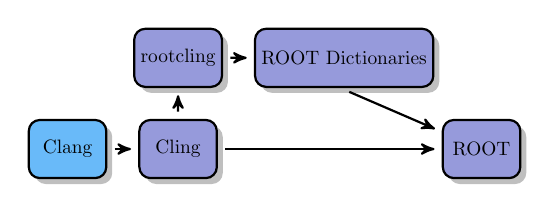
\begin{tikzpicture}[outer sep=0.05cm, node distance=0.8cm, scale=0.7, transform shape]
        
    \node[model, fill=my_lightblue, name=clang] (clang) {Clang};
    \node[model, fill=my_purple, name=cling, right=0.5cm of clang] (cling) {Cling};
    \node[model, fill=my_purple, name=rootcling, above=0.5cm of cling] (rootcling) {rootcling};
    \node[model, fill=my_purple, name=dicts, right=0.5cm of rootcling] (dicts) {ROOT Dictionaries};
    \node[model, fill=my_purple, name=root, right=4cm of cling] (root) {ROOT};

    \draw[line, ->] (clang.east) -- (cling);
    \draw[line, ->] (cling.north) -- (rootcling);
    \draw[line, ->] (rootcling.east) -- (dicts);
    \draw[line, ->] (dicts.south) -- (root);
    \draw[line, ->] (cling.east) -- (root);
    
  \end{tikzpicture}
  \caption{Dependency Graph of C++ Modules in ROOT}
  \label{fig:pchandpcm}
\end{figure}


\begin{listing}[h]
    \noindent
    \begin{minipage}[h]{\textwidth}
    \begin{cppcode*}{}
// Foo.h
    |\label{line:foobar}|namespace foo { struct bar{}; }
    |\label{line:structs}|struct S{};

// libFoo.rootmap
    |\label{line:decls}|{ decls }
    namespace foo { }
    struct S;
 
    |\label{line:libfoo}|[ libFoo.so ]
    # List of selected classes
    class bar
    struct S

// G__Foo.cxx (aka libFoo dictionary)
    namespace {
      void TriggerDictionaryInitialization_libFoo_Impl() {
        static const char* headers[] = {"Foo.h"}
        // More scaffolding
        extern int __Cling_Autoloading_Map;
        namespace foo{struct __attribute__((annotate("$clingAutoload$Foo.h"))) bar;}
        struct __attribute__((annotate("$clingAutoload$Foo.h"))) S;
       // More initialization scaffolding.
    }
    \end{cppcode*}
    \end{minipage}
    \caption{Example of ROOT dictionary for libFoo.}
    \label{list:foo}
\end{listing}

\section{Background}

\section{Implementation}
\label{implementation}

An implementation of the C++ modules concept itself exists in the LLVM frontend Clang \cite{clang-modules-doc} which is used as a library by ROOT. Clang supports the Modules TS and hosts modules research and development work. Clang's implementation encourages incremental, bottom-up adoption of the C++ modules \cite{Smith-cppcon}. The implementation is designed to work for C, C++, ObjectiveC, ObjectiveC++ and Swift \cite{Moduralize-doc}. Users can enable the modules feature without modifications in header files. Clang allows users to specify module interfaces in a dedicated file, called module maps files. A module map file expresses the mapping between a module file and a collection of header files. It can be mounted using the compiler’s virtual file system overlay mechanism to non-writable library installation paths. In practice, a non-invasive modularization can be done easily by introducing a module map file. In some cases the module map files can be automatically generated if the build system knows about the list of header files in every package.

Several steps were taken to adopt C++ modules in ROOT. First, we supported compiling ROOT with C++ modules. It halfed ROOT's compilation time. This effort includes generating module map files and resolving cyclic header dependency inside ROOT. Next, we taught rootcling dictionary generator to generate PCM files attached with I/O information. We taught ROOT to preload all PCMS at the startup time in order to make declaration available without \#including the appropriate headers. Also, we implemented the autoloading of libraries in ROOT which is not depending on old infrastructure (ROOTMAPS), which gives correctness benefits shown in section \ref{correctness} and is efficient compared to ROOTMAPS.

For the C++ modules adoption in experiments, we have been working closely with CMSSW team \cite{cms}. ROOT can already be compiled with runtime C++ in CMS environment, and we will enable PCM generation for their libraries one by one. We can gradually migrate dictionary generation to PCM, as our current implementation falls back to ROOTMAP when a PCM is not generated. It enables us to incrementally migrate from the old to the new infrastructure.

\section{Results}
\label{results}

\subsection{Performance Results}

\section{Limitations and Future work}

\section{Acknowledgments}

This work has been supported by an Intel Parallel Computing Center grant, by U.S. National Science Foundation grants PHY-1450377, OAC-1450377 and PHY-1624356, and by the U.S. Department of Energy, Office of Science.

The authors would like to thank CERN/EP-SFT and the ROOT team in particular.


\section*{References}

\begin{thebibliography}{10}
\bibitem{vassil-paper}
Vassil Vassilev, J. Phys.: Conf. Ser. \textbf{898}, 072023 (2017)

\bibitem{clang-modules-doc}
Clang Modules Documentation, \url{http://clang.llvm.org/docs/Modules.html}, accessed: 2018-24-11

\bibitem{Moduralize-doc}
Modularize Documentation, \url{http://clang.llvm.org/extra/modularize.html}, accessed: 2018-24-11

\bibitem{Gregor-cppcon}
Doug Gregor, cppCon 2016, Modules, URL \url{http://llvm.org/devmtg/2012-11/#talk6}

\bibitem{Klimek-cppcon}
Manuel Klimek, cppCon 2016, Deploying C++ Modules to 100s of Millions of Lines of Code, URL \url{https://cppcon2016.sched.com/event/7nM2/deploying-c-modules-to-100s-of-millions-of-lines-of-code}

\bibitem{Smith-cppcon}
Richard Smith, cppCon 2016, There and Back Again: An Incremental C++ Modules Design, URL \url{https://cppcon2016.sched.com/event/7nM6/there-and-back-again-an-incremental-c-modules-design}

\bibitem{David-talk}
David Blaikie, LLVM developer's meeting 2018, Build Impact of Explicit and C++ Standard Modules, URL \url{https://youtu.be/b-iiA18BRCQ}

\bibitem{rootbench}
Oksana Shadura, CHEP 2018 preprint, Continuous Performance Benchmarking Framework for ROOT

\bibitem{cms}
CMS Collaboration, “The CMS experiment at the CERN LHC”, JINST 3 (2008) S08004. doi:10.1088/1748-0221/3/08/S08004.

\end{thebibliography}

\end{document}